\documentclass[12pt]{article}
\usepackage{textcomp}
\usepackage{underscore}
\usepackage{amsmath}

% Formatting packages
\usepackage[margin=1.0in]{geometry}
\usepackage[utf8]{inputenc}
\usepackage{setspace}
\usepackage{indentfirst}

\usepackage{graphicx}
\graphicspath{ {images/} }

% Below stuff is all used for making highlighted code snippets
\usepackage{listings}
\usepackage{color}
\definecolor{dkgreen}{rgb}{0,0.6,0}
\definecolor{gray}{rgb}{0.5,0.5,0.5}
\definecolor{mauve}{rgb}{0.58,0,0.82}
\lstset{frame=tb,
  language=Python,
  aboveskip=3mm,
  belowskip=3mm,
  showstringspaces=false,
  columns=flexible,
  basicstyle={\small\ttfamily},
  numbers=none,
  numberstyle=\tiny\color{gray},
  keywordstyle=\color{blue},
  commentstyle=\color{dkgreen},
  stringstyle=\color{mauve},
  breaklines=true,
  breakatwhitespace=true,
  tabsize=3
}


\newcommand{\mytitle}{\textbf{An Automatic Grader for Embedded Systems Courses}}
\newcommand{\mydate}{August 18, 2017}

\begin{document}

\begin{titlepage}

\centering
\mytitle \\
\vspace{12pt}
by Daniel Mendelsohn \\
MIT S.B., 2015 \\
\vspace{12pt}
Submitted to the \\
Department of Electrical Engineering and Computer Science \\
in Partial Fulfillment of the Requirements for the Degree of \\
\vspace{12pt}
Master of Engineering in Electrical Engineering and Computer Science \\
\vspace{12pt}
at the \\
\vspace{12pt}
Massachusetts Institute of Technology \\
\vspace{12pt}
August 2017 \\
\vspace{12pt}
\textcopyright \hspace{0.05in} Massachusetts Institute of Technology 2017.  All rights reserved. \\
\vspace{48pt}

Author \dotfill \\
\begin{flushright}
Department of Electrical Engineering and Computer Science \\
\mydate
\end{flushright}
\vspace{36pt}

Certified by \dotfill \\
\begin{flushright}
Joseph Steinmeyer \\
Thesis Supervisor \\
\mydate
\end{flushright}
\vspace{24pt}

Accepted by \dotfill \\
\begin{flushright}
Dr. Christopher J. Terman \\
Chairman, Masters of Engineering Thesis Committee
\end{flushright}

\end{titlepage}

\addtocounter{page}{1}

\newpage
\mbox{}
\newpage

\begin{center}
\mytitle \\
by \\
Daniel Mendelsohn \\
\vspace{12pt}
Submitted to the Department of Electrical Engineering and Computer Science\\
 on \mydate{}, in Partial Fulfillment of the Requirements for the Degree of\\
 Master of Engineering in Electrical Engineering and Computer Science
\end{center}
\vspace{12pt}
\textbf{ABSTRACT} \\

\noindent In this thesis, we introduce MicroGrader, an automated grader for embedded systems projects.  The grader runs on a laptop or desktop computer, while the embedded system being evaluated runs on a microcontroller.  By implementing a custom communication protocol between the grader and the embedded system, we enable the grader to inject test inputs and observe the resulting outputs.

We describe a specification format for instructors to define the technical requirements of an assignment.  This format is meant to be simple to use, but highly expressive to allow for a wide range of possible assignments.  We also outline the implementation of the MicroGrader system and the underlying communication protocol.  We discuss the constraints that the specification format and the technical implementation impose on instructors.  Finally, we describe a method to automatically generate specifications using a staff-built reference solution for a generic assignment. 

\newpage
\mbox{}
\newpage

\tableofcontents

\doublespacing

\newpage
\section{Introduction}
Verification of program behavior has been a major concern for engineers and academics since the early days of computing.  The study of software testing has grown into a significant field of computer science.  In this thesis, we will describe a software tool (``MicroGrader") that verifies the correctness of embedded systems, specifically in an educational context.  Essentially, it is an automated grader for embedded systems assignments that provides actionable feedback to students.

We must understand why the verification of an embedded system requires a specialized approach, and understand how the educational context affects design choices.

First, let's discuss program verification in general, at a high level. In order to assess the correctness of any software system, we must first choose how to model such a system.  Often, it is useful to model a software system as a finite state machine (FSM).  That is, at any time, the output and next state of the system are uniquely defined by the input and current state of the system.  Two FSMs are considered equivalent if they produce an identical sequences of outputs for the same sequence of inputs.  If we only care about the functional correctness of a system, we should consider any FSMs that are equivalent to the correct ``solution" to be correct as well.  This implies we should only evaluate the output sequences and not the internal state.

While it is possible to exhaustively verify a black-box FSM, the number of steps required to do so is hyper-exponential, making this infeasible in practice.  Rather, we typically test FSMs by verifying that they produce the correct output sequence for a useful subset of the possible input sequences.  That useful subset of inputs is often chosen manually.  The correct outputs might be defined manually as well.  In the context of education, it is easier to use a ``staff solution" to define the outputs.  That is, the staff solution is canonically considered correct, and student solutions must match the output of the staff solution to be considered correct.
   
In most cases, the evaluator and the evaluated system can run on the same computing platform (e.g. an x86 processor with a compiler/interpreter for the relevant language).  Typically, the evaluator exerts direct control over the evaluated system.  For embedded systems, the resource constraints of a microcontroller -- both in terms of memory and speed -- force us to separate the the evaluator and the evaluated system.  In the case of MicroGrader, the evaluator is a Python program running on a full-fledged processor, while the evaluated systems are embedded programs.

This separation of evaluator and the evaluatee (an embedded system in our particular case) is the primary focus of this paper, and it presents some new challenges.  The evaluator requires the ability to specify the inputs to the embedded system, which are typically real-world sensor readings.  Furthermore, it requires the ability to observe the outputs of the embedded system, which are typically physical output indicators (e.g. a motor, LED, etc).  In MicroGrader, a communication protocol between the evaluator and the embedded system enables this access.  The protocol is designed to be minimally intensive for the embedded system.  Specifically, a low-level library on the embedded side implements one side of this protocol, which allows it to ``request" inputs from the evaluator rather than performing actual sensor sampling.  We can consider this an injection of test inputs.  This library also allows for the embedded system to report outputs.

Beyond the separation of evaluator and evaluatee, there are additional differences between evaluating embedded and non-embedded software.  Principal among these is the importance of timing.  While the specification of a non-embedded program \textit{could} include strict rules for the timing of specific operations, it's fairly unusual.  Existing automatic graders may consider the overall program running time, but very few graders delve into the fine timing details. In embedded systems, timing is often of paramount importance.  For example, in computing a single state update, an embedded system may require multiple inputs and produce multiple outputs.  The inputs are not sampled at the exact same time, and the outputs are not produced at the exact same time.  Furthermore, the implementation of the embedded program determines the timing of these events; an evaluator has no ability to compel the embedded system to sample an input at exactly time $X$ or produce an output at exactly time $Y$.

Our evaluator cannot control the timing of input and output (I/O) events, nor can it ignore the timing of those events.  This forces us to modify our ``pure" FSM model, where I/O events occur at discrete time intervals.  Rather than examining how an embedded system converts a set of discrete input sequences to a set of discrete output sequences, we must examine how it converts a set of continuous input signals to a set of continuous output signals.

The process of constructing test cases can be time-consuming.  It is often prohibitively tedious for instructors to specify all the test inputs and expected outputs.  Therefore, MicroGrader includes a feature for ``recording" the operation of an instructor's system, and using that recording to programmatically generate test inputs and expected outputs. 


\newpage
\section{Prior Work}
In my search for existing automatic graders for embedded systems courses, I found only one system that's actually being used.  The University of Texas at Austin (UT Austin) offers an EdX course "Embedded Systems - Shape The World" \footnote{https://www.edx.org/course/embedded-systems-shape-world-utaustinx-ut-6-10x}, which uses a grading system called TExaS.  Most of what I learned about TExaS was gleaned by examining the course on EdX itself; I was not able to find technical documentation.

TExaS consists of a grader running on a student's computer, that observes the activity of the student's microcontroller.  It is decidedly not multi-platform: the core of TExaS runs as a plug-in to the Keil Microcontroller Development Kit \footnote{http://www2.keil.com/mdk5/}, which only runs on Windows.  That plug-in works with the particular microcontroller used in the course.

The platform lock-in of TExaS has benefits.  It appears to have low-level access to the operation of the microcontroller and places little -- if any -- burden on the microcontroller itself.  TExaS can observe all the inputs and outputs of the microcontroller and it can even observe arrays of raw data in the microcontroller's memory.

TExaS does not inject test input values into the microcontroller.  Rather, test cases prompt the student to perform certain operations (e.g. press button connected to pin 5).  This reliance on interactivity and student control makes it difficult to construct complex test cases.  Most of the assignments graded by TExaS are fairly simple from an I/O perspective: the main output is a small array of light-emitting diodes (LEDs).  While I cannot speak to the usability on the instructor's side, the system seems to be limited in the scope of what it can do, but very capable of accomplishing grading tasks within that scope.

In designing and building MicroGrader, I wanted a cross-platform system to generalize the task of grading an embedded system.  Furthermore, I wanted a broader set of possible inputs and outputs, and the ability to grade more complex tasks.

In MIT's 6.S08 (Interconnected Embedded Systems), microcontroller grading is completely manual.  Students show instructors solutions in-person or by video.  This approach is time-consuming and does not scale well.  6.S08 uses CAT-SOOP \footnote{https://catsoop.mit.edu/} to evaluate certain software functions.  Students enter C++ code, which is then evaluated on the centralized course server and evaluated within the CAT-SOOP environment.  This allows the course staff to verify the student's code to some extent, but the execution of the code is inevitably different on the actual microcontroller.  Students often find that solutions that work in the CAT-SOOP checker, fail on the microcontroller.

\newpage
\section{Motivating example: ``Wikipedia Scroller"}
\label{sec:wiki-scroller}
Before diving into technical details of the automated grader, it helps to have a motivating example in mind;  MIT's 6.S08 includes an exercise called ``Wikipedia Scroller", in which students build a digital encyclopedia using a microcontroller, a push-button switch, a nine-axis inertial measurement unit (IMU) and a 128x64 organic light-emitting diode (OLED) display.

Each student implements a tilt-based interface that allows the device's user to build an alphanumeric query string.  Using the ESP8266 chip, the device transmits the query string to a server-side Python program.  That Python program uses the query string to formulate a query to the Wikipedia API, parses the response from the Wikipedia API, and transmits the first 200 characters of the relevant Wikipedia description to the embedded device.

\begin{figure}[h]
\centering
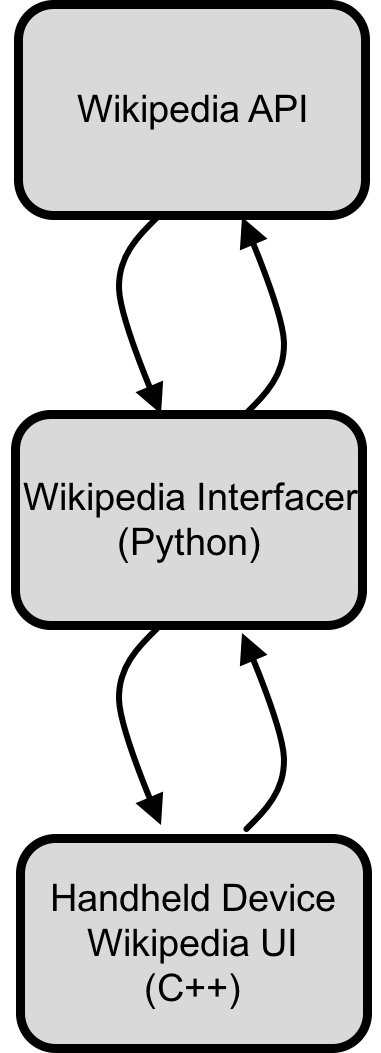
\includegraphics[scale=0.5]{wiki-block-diagram.png}
\vspace{5mm}
\caption{Block diagram for Wikipedia Scroller. Bottom block is the embedded system.}
\end{figure}


\subsection{Specification for the embedded system}
The embedded device allows its user to construct an alphanumeric query string, and it displays the results of the corresponding query.  The primary input mechanism is ``tilt", as measured by accelerometer readings.  In addition, the user can perform two actions using the push-button switch.  We define a press to be a \textit{short press} if its duration is under one second.  We define a press to be a \textit{long press} if its duration is at least one second.  The system can be viewed as an FSM with three states.  Note that, in the specifications for each state below, some of the finer details have been omitted in this paper for the sake of brevity.

\subsubsection{State 0: display state}
In this state, the result for the most recent query should be displayed.  Specifically, the screen should show as many characters as possible from the most recent HTTP response.  Initially, before any query has occurred, we define the ``most recent result" to be the empty string.  The system's built-in 5x7 fixed-size font should be used, so that eight lines, each comprised of 21 characters, can fit on the screen.  See Figure \ref{fig:pigeons} for an example.  When the user performs a long press, the system should switch to the query entry state.

TODO: replace Figure \ref{fig:pigeons} with a better photo, without html tag

\begin{figure}[t]
\centering
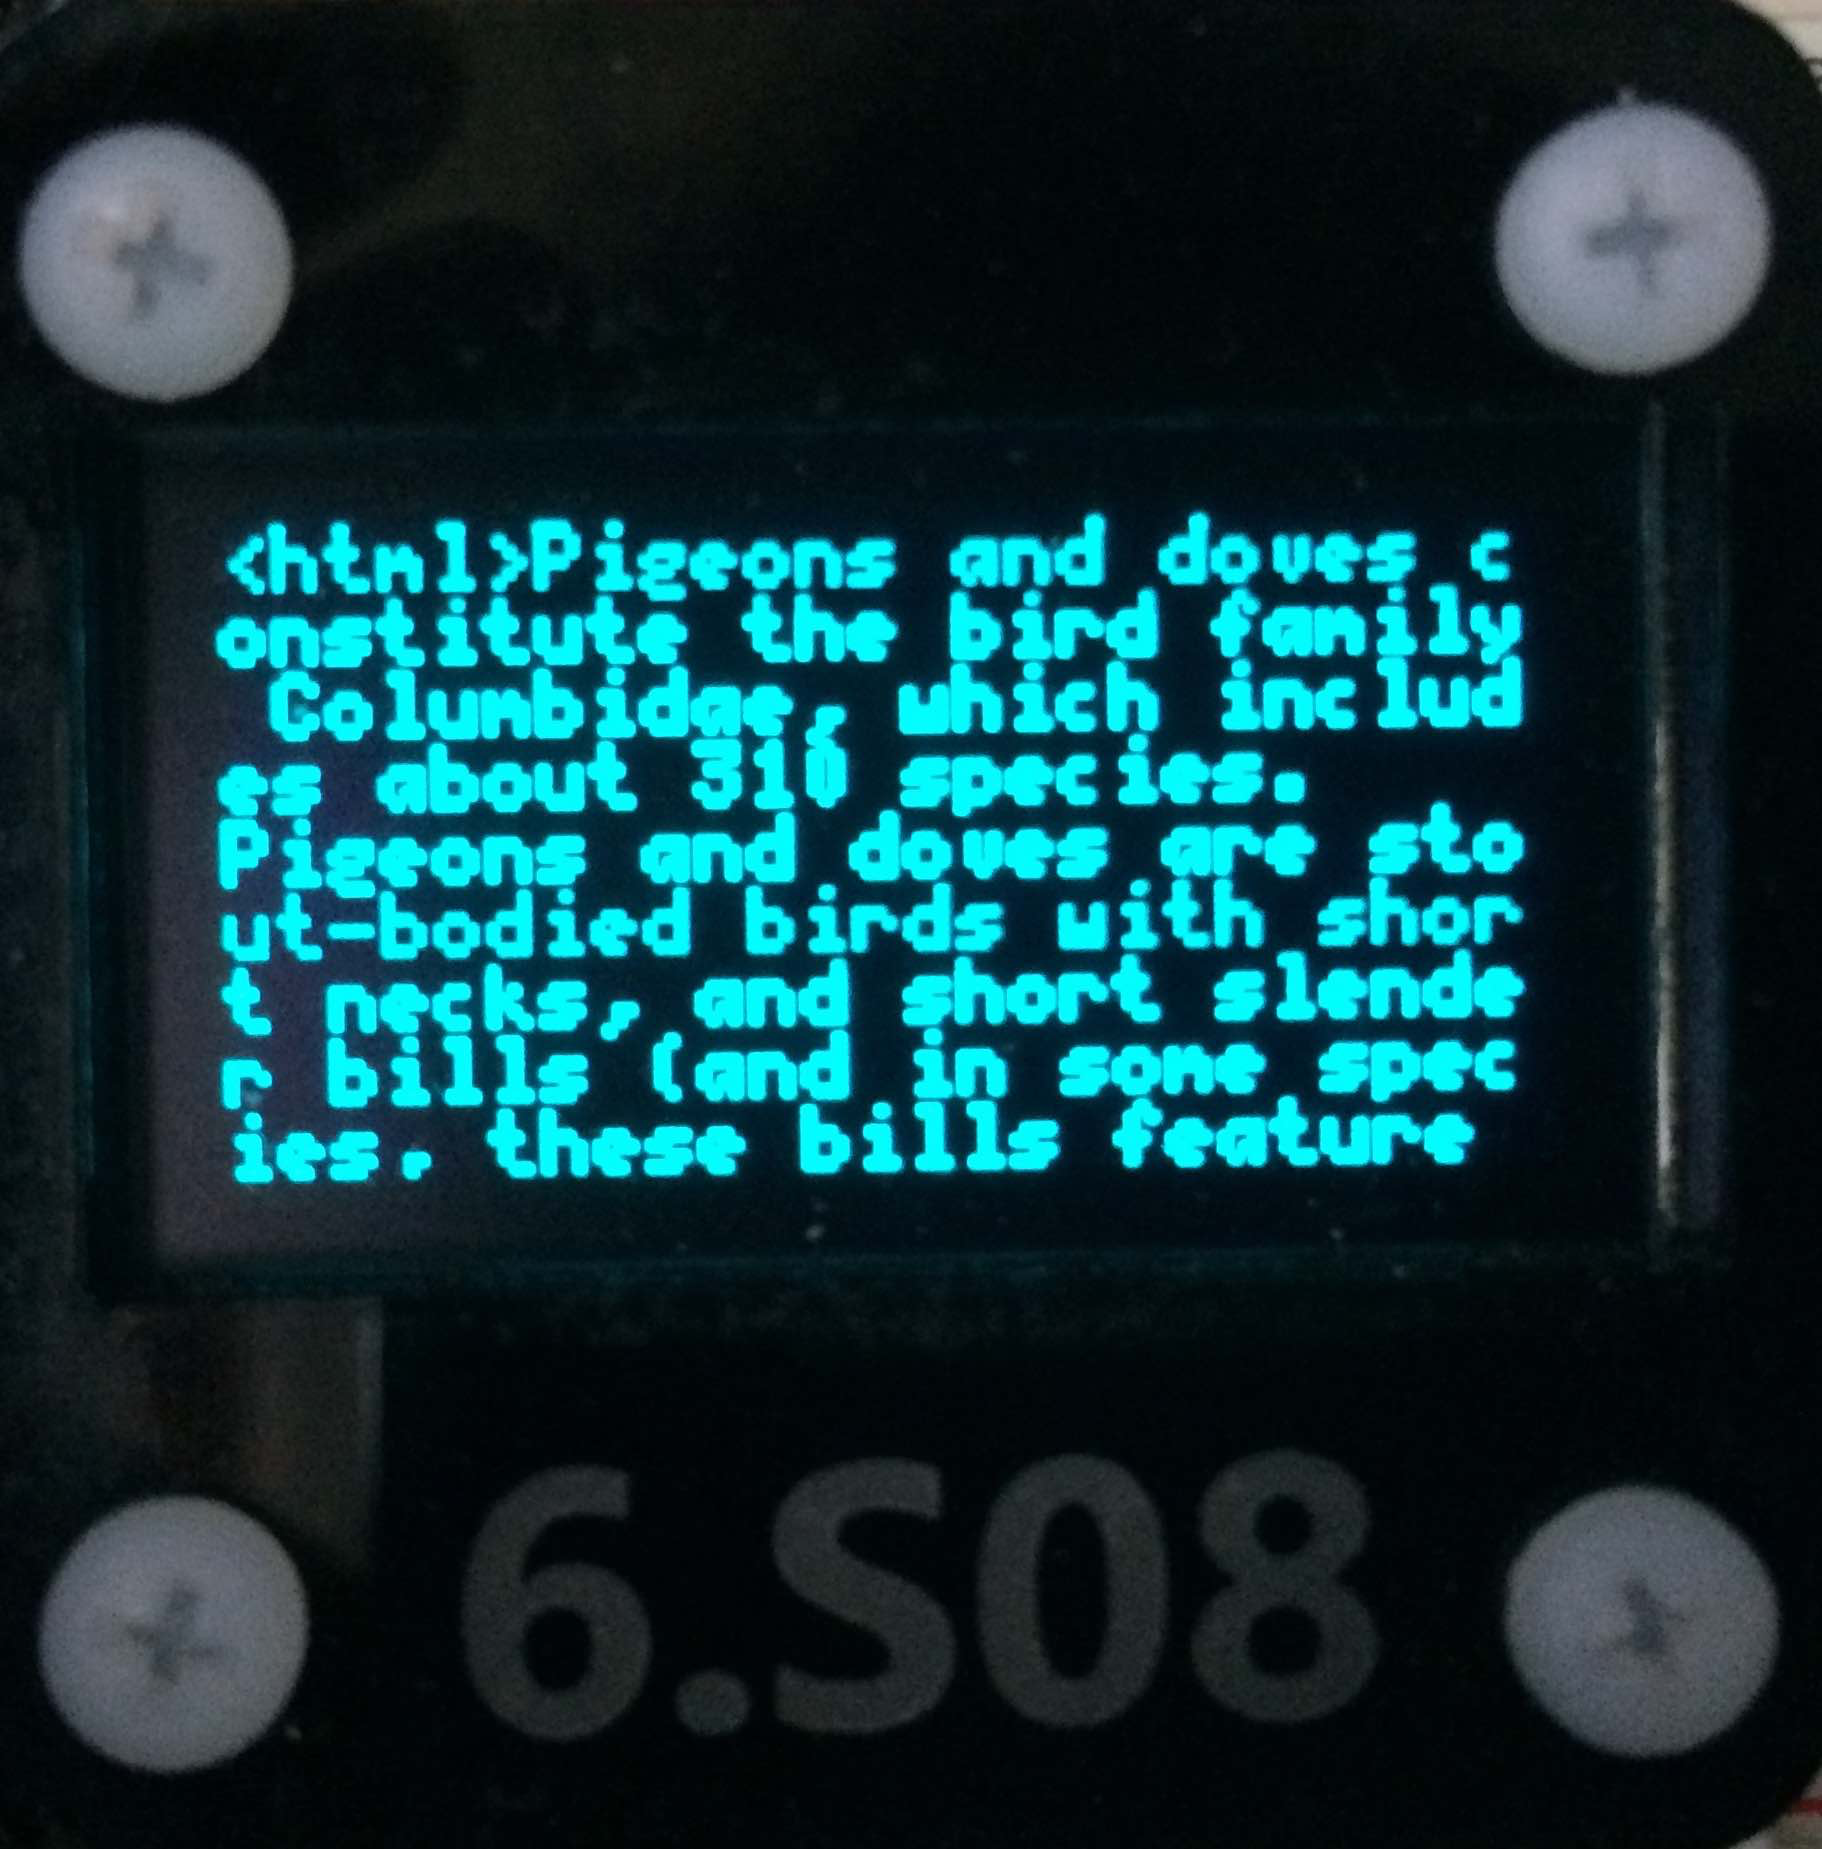
\includegraphics[scale=0.125]{pigeons.png}
\vspace{5mm}
\caption{Screen output when in the display state. The last query was ``pigeons".}
\label{fig:pigeons}
\end{figure}

\subsubsection{State 1: query entry state}
In the query entry state, there are two relevant variables: \texttt{query} and \texttt{next_char_index}.  Initially, \texttt{query} is the empty string, and \texttt{next_char_index} is 0.  By definition, we say that the ``next character" is the character in the string

\begin{centering}
\texttt{"abcdefghijklmnopqrstuvwxyz0123456789"}\\
\end{centering}
\noindent at position \texttt{next_char_index}.  So, the next character is initially \texttt{"a"}.

In order to build the query string, the user selects characters one by one.  The user tilts the device left and right to ``scroll" through the possible options for the next character.  If the device is tilted $20^{\circ}$ to the right, then \texttt{next_char_index} should increment every 150 milliseconds.  If the device is tilted $20^{\circ}$ to the left, then \texttt{next_char_index} should decrement every 150 milliseconds.  The index should wrap around, so that \texttt{"9"} and \texttt{"a"} are essentially adjacent characters.

With a short press, the user ``locks in" the next character.  That is, the next character should be appended to the query string, and then \texttt{next_char_index} should be reset to 0.  Finally, with a long press, the user finishes the construction of the query string, which is then transmitted via HTTP to the server-side portion of the project.

In this state, the text on the OLED screen should always be \texttt{query}, plus the next character.  For example, if \texttt{query} is \texttt{"pigeo"} and \texttt{next_char_index} is 0, then the string \texttt{"pigeoa"} should be displayed on the screen.

TODO: add some demonstration photos

\subsubsection{State 2: waiting state}
In this state, the device waits for a response from the server.  When the response arrives, the system should transition back to the display state (which is responsible for displaying the response).  In this state, the OLED screen should contain the text \texttt{"Waiting for response"}.

\subsection{Manually grading Wikipedia Scroller}
As a teaching assistant (TA) grading 6.S08 assignments, the author performed the following procedure to check that the assignment was implemented correctly.

First, upon system initialization, he checked that the OLED screen was blank.  Then, he performed a long press to transition to the query entry state and verified that the character \texttt{"a"} appeared on the screen.  He then tilted the device slightly left and right (less than $20^{\circ}$) to ensure the text did not change, signifying that the scroller was not too sensitive to tilt.  He would then increase the tilt to more than $20^{\circ}$ to ensure that scrolling occurred.  When holding a constant tilt at a high angle, he checked the rate at which the character changed.  He also checked that wrap-around was correctly implemented in both directions (i.e. that a left tilt from \texttt{"a"} yielded \texttt{"9"} and that a right tilt from \texttt{"9"} yielded \texttt{"a"}.

After verifying that the scrolling behavior was correct, he entered a short query string to ensure that string-building worked.  He performed a long press to send the query to the server and checked that the proper response appeared on the screen shortly thereafter.  Finally, he performed a long press to prompt a transition to query entry mode again, and verified that the old query had been cleared and the screen showed just \texttt{"a"}.

In this manner, the author was able to grade each student's work in under two minutes.  In a class of 180 students, six hours of grading time was required for this assignment alone.  Furthermore, it was difficult to give students detailed feedback, and students only received feedback after it was too late to fix any mistakes.  An automated grader would solve these problems.

\newpage
\section{Defining a test}
In this chapter, we describe the design of the \textit{test case} data structure, and explain the reasoning behind it.  At an abstract level, a grader's role is to assign a score to an embedded system.  A human grader might rely on intuition or a checklist in order to assign a score.  For MicroGrader, the test case defines the process by which a score is assigned.  A MicroGrader test case serves two primary functions.  First, it specifies any necessary input signal signals.  Second, it specifies how the resulting output signals should be graded.

\subsection{The shortcomings of statically defined inputs}
While developing MicroGrader, we first explored a static approach to specifying inputs.  In this design, all input signals would be completely predefined.  For example, a test case could specify a digital input as seen in Figure \ref{fig:static-input}.

\begin{figure}[ht]
\centering
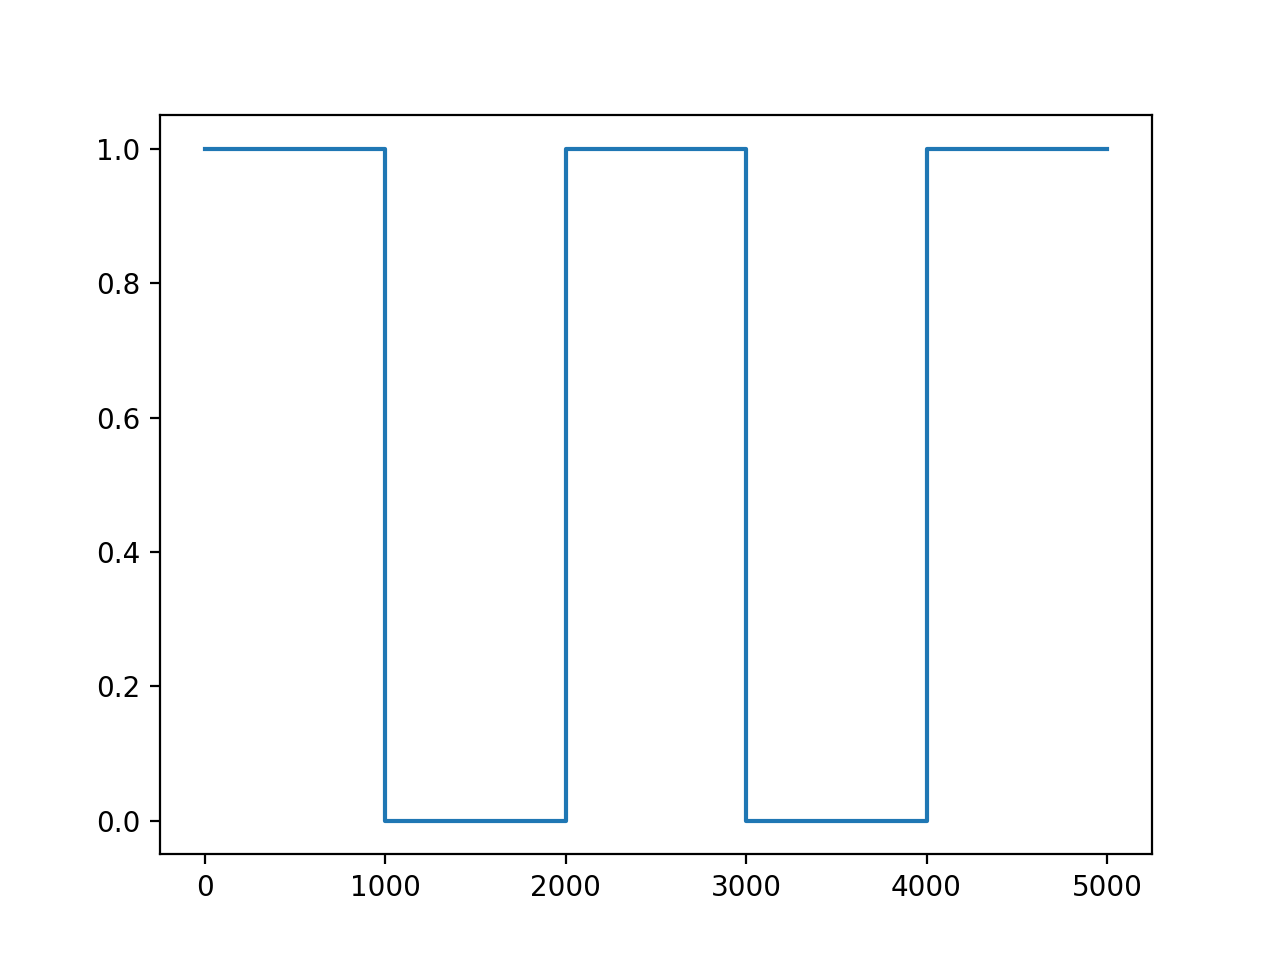
\includegraphics[scale=0.75]{button-signal.png}
\vspace{5mm}
\caption{A simple digital signal.}
\label{fig:static-input}
\end{figure}

In this particular example, presuming the digital input is connected to an active-low push-button switch, the test case indicates the button is pressed in the interval $[1000,2000)$ and $[3000,4000)$ and not pressed at all other times.  We would define $t=0$ as the time at which the microcontroller last powered on or reset.  In this static paradigm, the input signals would not depend upon the behavior of the embedded system.

In practice, we found that statically defined inputs limited scope of assignments for which MicroGrader could be used.  Grading assignments often requires input signals that are dependent on the behavior of the system.  Consider ``Wikipedia Scroller" for a concrete example.  In particular, Wikipedia Scroller requires that the system wait for an HTTP response after transmitting a query.  The length of time spent waiting for the response varies widely and is not within the student's control.  When human graders evaluate the system, they know to wait for the Wikipedia text to appear (indicating an HTTP response has arrived), before performing additional test actions.  The HTTP response might arrive less than a second after the request, or it might arrive several seconds later.  We should consider the timing of subsequent actions relative to the arrival of the HTTP response, not relative to the initialization of the system as a whole.  We can conclude that, in order to effectively grade Wikipedia Scroller, MicroGrader test cases need to dynamically define inputs, with respect to run-time events.  More generally, dynamically defined inputs allow MicroGrader to deal with variable latencies that are not within the student's control.

\subsection{Dynamically defined inputs}
We have established that MicroGrader must dynamically generate microcontroller inputs, based on the previous activity of the embedded system.  Human graders can only use system outputs to determine future input actions.  An automated grader could go further, relying on internal embedded system events in addition to system outputs.  For Wikipedia Scroller, human graders use the appearance of Wikipedia text to indicate that the HTTP response has arrived; an automated grader could, in principal, observe the arrival of the HTTP response directly and not rely on an indirect indicator.

Observing internal events directly can simplify the logic for test cases.  It is important to carefully decide which internal events MicroGrader should observe; since the grader is remotely assessing embedded system, it is impractical to observe low-level events that occur frequently.  In the current implementation of MicroGrader, the observed internal events are: ``system initialized", ``Wifi connected", ``HTTP request sent", ``HTTP response received", and ``GPS fix acquired".  In addition, MicroGrader supports a ``print" event, which allows the embedded system to send a string to the automated grader.  In general, we define a MicroGrader \textit{observation} to be one of these internal events or any external output.

\subsubsection{Data structure: ``Condition"}
\label{sec:condition}
We want the ability to specify the timing of system inputs relative to a specific, unique event that occurs during the execution of an embedded system.  In order to specify unique run-time events, we must first introduce a data structure that describes those events.  We will refer to this data structure as a \textit{condition}.  As an embedded system executes a program, MicroGrader can determine the condition's $t_{\text{satisfied}}$, the elapsed time between the embedded system's initialization and the condition's satisfaction.  A condition's $t_{\text{satisfied}}$ can be undefined, signifying that the condition was never satisfied during the embedded system's execution.

Our condition data structure can express unique events such as: ``The first HTTP request", ``the second HTTP request", and ``the first time that the word `cat' appears on the embedded display".  It achieves this with a recursive design; complex conditions can be built by composing simpler ones.  There are four fundamental types of conditions.

The first type of condition is the \textit{basic condition}.  A basic condition's $t_{\text{satisfied}}$ is defined by a \textit{cause}. A cause is boolean function that takes a single input representing a MicroGrader observation.  As MicroGrader processes each observation during the execution of an embedded program, the cause function is invoked with that observation as its input.  The condition's $t_{\text{satisfied}}$ is the \textbf{first} time at which the cause function returns \texttt{true}.  For example, we can describe ``the first HTTP request" using a basic condition; the cause function would return \texttt{true} if and only if the observation is an HTTP request.

The second type of condition is the \textit{after condition}.  After conditions have another condition (of any kind) as a ``precondition".  Like basic conditions, after conditions have a cause function.  This cause function is only invoked for observations that occur after the precondition is satisfied.  As before, the after condition's $t_{\text{satisfied}}$ is the first time at which the cause function returns \texttt{true}.  We can describe ``the second HTTP request" using this type of condition.  In particular, the precondition would be a condition signifying ``the first HTTP request", as described above.  The cause function would return \texttt{true} if any only if the observation is an HTTP request.  Note that this condition has the same cause function as the condition for ``the first HTTP request", the existence of a precondition is the only difference.  In a similar manner, we could define the nth occurrence of any event.

Alternatively, the cause of an after condition can be a single number, $t_{\text{cause}}$, instead of a function.  In this case, we consider this condition's $t_{\text{satisfied}}$ to be the precondition's $t_{\text{satisfied}}$ plus $t_{\text{cause}}$.  In general, an after condition cannot be satisfied without its precondition being satisfied.

The third type of condition is the \textit{and condition}.  This type of condition has no \textit{cause}, but rather a set of subconditions, which can be of any condition type.  This condition is considered to be met once \textbf{all} of the subconditions are met.  Equivalently, this condition's $t_{\text{satisfied}}$ is the maximum of its subconditions' $t_{\text{satisfied}}$ values, or undefined if any subcondition has an undefined $t_{\text{satisfied}}$.

The fourth and final type of condition is the \textit{or condition}.  It is analogous to the \textit{and condition}, except it is considered to be satisfied once \textbf{any} of its sub-conditions are met. Equivalently, this condition's $t_{\text{satisfied}}$ is the minimum of its subconditions' $t_{\text{satisfied}}$ values, or undefined if all subconditions have an undefined $t_{\text{satisfied}}$.

In Tables \ref{table:observations}, \ref{table:conditions}, and \ref{table:condition-descs}, we examine a concrete example showing a sequence of observations and a set of conditions, including each condition's value for $t_{\text{satisfied}}$ with respect to this set of observations.  Here, $f_{\text{httpreq}}$ and $f_{\text{high}}$ are cause functions, which take a single observation as input.  In particular, $f_{\text{httpreq}}$ returns \texttt{true} if the observation represents the sending of an HTTP request, and $f_{\text{high}}$ returns \texttt{true} if the observation represents the setting of digital output 13 to 1.  Notice that condition 4 is satisfied at $t=4000$, since both its subconditions are satisfied and the maximum of the subconditions' $t_{\text{satisfied}}$ is 4000.  By contrast, condition 5 is never satisfied since its cause function is only invoked for observations 5, 6, and 7.

\begin{table}
\begin{center}
\caption{Example observations}
\label{table:observations}
\begin{tabular}{l|lr}
& Description & Timestamp (ms) \\ \hline
Observation 1 & System initialization & 0 \\
Observation 2 & Digital output 13 set to 1 & 1000 \\
Observation 3 & HTTP request sent & 2000 \\
Observation 4 & HTTP response received & 3000 \\
Observation 5 & HTTP request sent & 4000 \\
Observation 6 & HTTP response received & 5000 \\
Observation 7 & Digital output 13 set to 0 & 6000 \\ \hline
\end{tabular}

\vspace{5mm}

\caption{Example conditions, with $t_{\text{satisfied}}$ calculated with respect to Table \ref{table:observations}}
\label{table:conditions}

\vspace{3mm}

\begin{tabular}{l|llllr}
& Type & Cause & Precondition & Subconditions & $t_{\text{satisfied}}$ (ms) \\ \hline
Condition 1 & Basic & $f_{\text{httpreq}}$ & N/A & N/A & 2000 \\
Condition 2 & After & $f_{\text{httpreq}}$ & Condition 1 & N/A & 4000 \\
Condition 3 & Basic & $f_{\text{high}}$ & N/A & N/A & 1000 \\
Condition 4 & And & N/A & N/A & Conditions 2 \& 3 & 4000 \\
Condition 5 & After & $f_{\text{high}}$ & Condition 2 & N/A & Undefined \\ \hline
\end{tabular}

\vspace{5mm}

\caption{Text descriptions of example conditions from Table \ref{table:conditions}}
\label{table:condition-descs}

\vspace{3mm}

\begin{tabular}{l|l}
& Description \\ \hline
Condition 1 & First HTTP request sent \\
Condition 2 & Second HTTP request sent \\
Condition 3 & Digital output 13 has been set to 1 \\
Condition 4 & Digital output 13 has been set to 1 and second HTTP request sent \\
Condition 5 & Digital output 13 has been set to 1 after second HTTP request sent \\ \hline
\end{tabular}
\end{center}
\end{table}

\subsubsection{Data structure: ``Input Frame"}
Now that we have a structure for specifying run-time events, we can describe input signals relative to such events.  To do so, we introduce a new data structure called the \textit{input frame}.  An input frame consists of a start condition, an end condition, and a \textit{value generator function}.  We will refer to the start condition's $t_{\text{satisfied}}$ as $t_{\text{start}}$, and the end condition's $t_{\text{satisfied}}$ as $t_{\text{end}}$.  We say that an input frame is \textit{active} in the time interval $[t_{\text{start}}, t_{\text{end}})$.

The value generator function has two inputs: a channel, $c$, and time, $t$.  The channel, more specifically, is an input channel such as ``analog input 5" or ``accelerometer x-axis".  The value generator function returns a valid value for channel $c$ (i.e. a float for an analog channel, or $\{0,1\}$ for a digital channel).  We interpret this returned value to be the value of the input signal on channel $c$ at time $t_{\text{start}}+t$.  The value generator function should be defined for all input channels used in the exercise, and for all $t>0$.

In the context of the Wikipedia Scroller exercise, we consider an example input frame.  Suppose the frame's start condition is ``system initialization" and the end condition is ``the first HTTP request".  The two-channel value generator function, shown in Figure \ref{fig:value-gen}, specifies the input signals relative to $t_{\text{start}}$.  When a properly designed ``Wikipedia Scroller" system processes those input signals, it should: start in the display state (with a blank screen), transition to the query entry state after the long button press, scroll through a few letters due to the subsequent tilting, lock in the selected letter due to the short press, and send the one-character query string to the project's backend due to the final long press.  This process supposes a certain orientation for the IMU, which should be specified in the instructions for the exercise.

\begin{figure}[h]
\centering
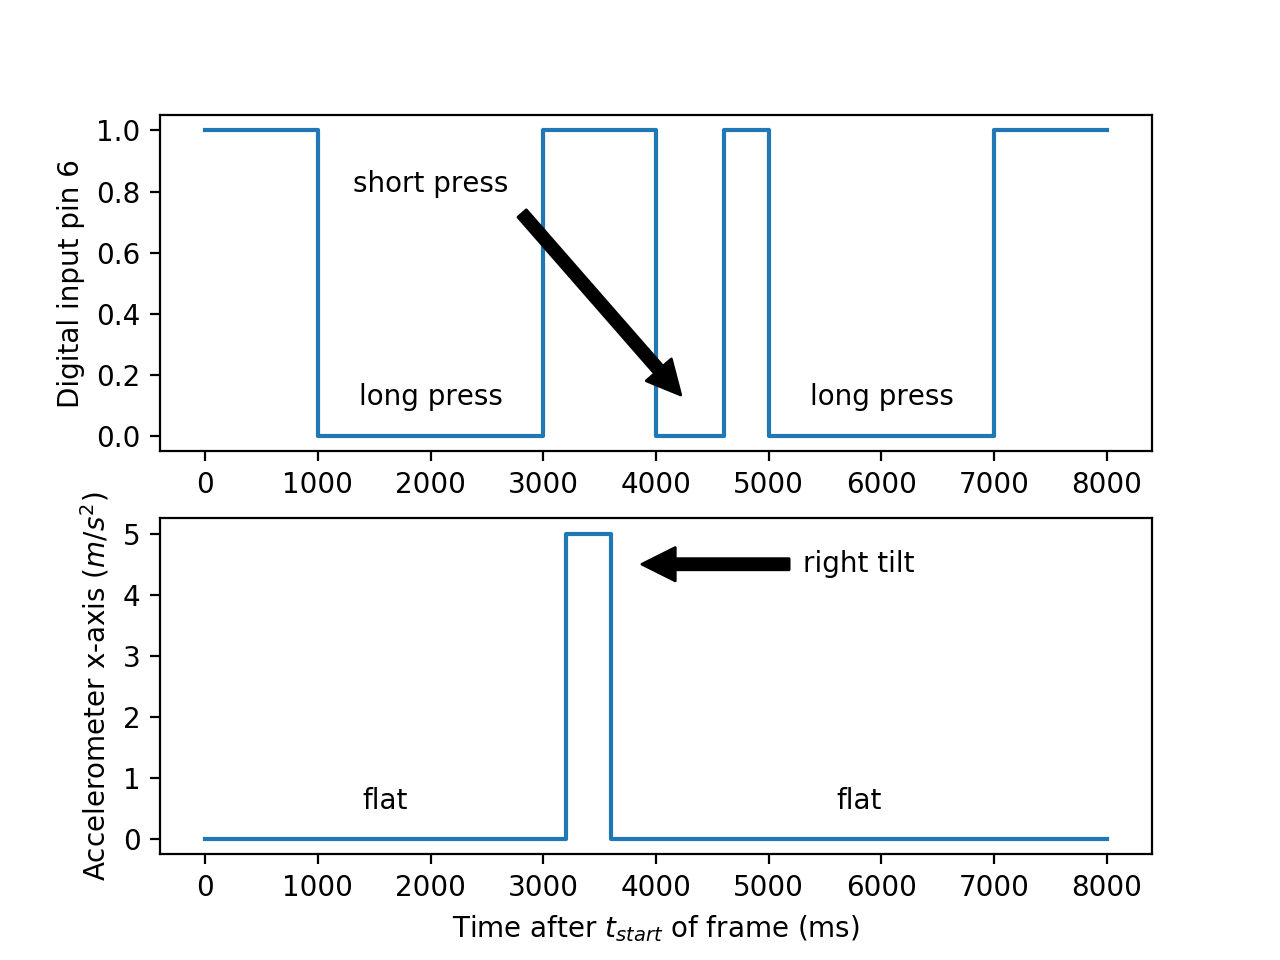
\includegraphics[scale=1]{wiki-frame.png}
\vspace{5mm}
\caption{Value generator function with two input channels.}
\label{fig:value-gen}
\end{figure}

\subsubsection{Determining input values}
A single test case usually contains multiple input frames.  At any time, MicroGrader might need to inject an input value into the embedded system.  If, at that time, a single input frame is active, we use that frame's value generator function to determine the value to inject.  We must consider the possibility that multiple input frames are active at the same time, as well as the possibility that no input frames are active.

If multiple input frames are active, we must choose which one determines the injected input value.  For this purpose, we add another attribute called \textit{priority} to our input frame data structure.  The highest priority active frame is used to determine the injected input value.  If there is a tie for the highest priority, the frame with the latest $t_{\text{start}}$ is used.  MicroGrader can be configured to instead use the frame with the earliest $t_{\text{start}}$ in a tie-breaker scenario.

If MicroGrader needs to inject an input value, and there are no active input frames, then a default value is used.  An instructor can specify a default value for any input channel.  In the case of an active-low push-button switch, it typically makes sense to use 1 as a default, indicating an unpressed button.  In the case of accelerometer readings, an instructor might want to use a default of 0 $\text{m}/\text{s}^2$ for two of the axes, and a default of 9.81 $\text{m}/\text{s}^2$ for the ``up-down" axis (due to gravity).

\subsection{Grading system outputs}
\label{sec:eval-point}
So far, we have established how MicroGrader specifies input values for a test case.  Now, we must describe how it grades the outputs of the embedded system.

MicroGrader has access to a sequence of output observations.  Output observations occur when the microcontroller generates an output.  For example, MicroGrader can observe the execution of a \texttt{digitalWrite} or \texttt{analogWrite} command on the Arduino platform, both of which specify an output voltage on a GPIO pin.  MicroGrader can also observe commands that change the embedded system's display.  Using this discrete set of output observations, MicroGrader recovers continuous output signals by assuming that outputs are constant until the next observation on the same channel.  Now, we need a method of grading a set of continuous output signals.


\subsubsection{Breaking up the grading task}
Let us consider a simple exercise, involving no inputs at all.  We will refer to this exercise as ``Blinky".  In this exercise, the microcontroller outputs a 1 Hz digital square wave on digital output 13, starting with a value of 0.  As graders, let us suppose that we only care to check the first two periods of this square wave; if these first two periods occur correctly, we will give the exercise full credit.

We define $t_{\text{start}}$ to be the time, in milliseconds, at which the embedded system finishes initializing.  Fundamentally, a grader performs four checks

\begin{itemize}
\item digital output 13 must have a value of 0 in the interval $[t_{\text{start}},t_{\text{start}}+500)$.
\item digital output 13 must have a value of 1 in the interval $[t_{\text{start}}+500,t_{\text{start}}+1000)$.
\item digital output 13 must have a value of 0 in the interval $[t_{\text{start}}+1000,t_{\text{start}}+1500)$.
\item digital output 13 must have a value of 1 in the interval $[t_{\text{start}}+1500,t_{\text{start}}+2000)$.
\end{itemize}

In the next section, we introduce a data structure called an \textit{evaluation point}, which can specify each of these four checks.

\subsubsection{Basic attributes of an evaluation point}
An evaluation point has a channel (digital output 13 in the example above) and an expected value.  It must also have an attribute that defines the time at which we expect this value.  To that end, an evaluation point has a time interval.

Since the timing of test inputs can be defined relative to run-time events, the timing of outputs can be sensitive to run-time events.  Therefore, an evaluation point also has a condition (as defined in section \ref{sec:condition}).  The evaluation point's time interval should be considered relative to the time at which the condition is met.

For ``Blinky", an instructor might consider using the four evaluation points described in Table \ref{table:blinky-basic-points} to assess a student's work.

\begin{table}[ht]
\begin{center}
\caption{A basic set of evaluation points for Blinky.}
\vspace{2mm}
\label{table:blinky-basic-points}
\begin{tabular}{c|cccc}
& Channel & Expected Value & Condition & Interval \\ \hline
Point 1 & Digital output 13 & 0 & System initialization & (0,500) \\
Point 2 & Digital output 13 & 1 & System initialization & (500,1000) \\
Point 3 & Digital output 13 & 0 & System initialization & (1000,1500) \\
Point 4 & Digital output 13 & 1 & System initialization & (1500,2000) \\ \hline
\end{tabular}
\end{center}
\end{table}

An evaluation point evaluates to either \texttt{true} or \texttt{false} with respect to a set of observed output signals.  There is no ``partial credit", since an evaluation point is our fundamental unit of grading.  If instructors want finer detail, they should create multiple separate evaluation points. 

\subsubsection{Augmenting the evaluation point for less restrictive specifications}
The evaluation points in Table \ref{table:blinky-basic-points} can verify that an embedded system implements the Blinky exercise.  In order to satisfy all four points, however, an implementation must be perfect.  That is, the rising and falling edges of the square wave must occur at exactly the correct times, to millisecond precision.  This rigidity is often undesirable in an educational context; some degree of lenience is often required in order for an academic course to avoid becoming bogged down with the finest details.

First, we augment the evaluation point data structure to allow for some timing flexibility.  Specifically, we add a new attribute called the \textit{required portion} (sometimes we will just refer to this attribute as the ``portion" for short), which is a float in the range $[0,1]$.  Using this attribute, we can relax the requirement that the student's system outputs have to be correct for the entire interval of an evaluation point.  Rather, the output value is only required to be correct for at least the specified (not necessarily contiguous) portion of the interval.  In an extreme case, a portion value of 1 implies the output must be correct for the whole interval.  At the other extreme, a portion value of $\epsilon$, a small positive value, implies the output must be correct at any time during the interval.  In our Blinky exercise, an instructor might decide to use 0.9 as the required portion, to allow for small deviations from the desired timing.

Second, we augment the evaluation point data structure to allow for value flexibility.  For certain output types, such as analog outputs, it is not appropriate to check for an exact output value.  Rather, it is usually desirable to allow for a range of allowable values.  We introduce the \textit{check function} attribute of an evaluation point to address this concern.  This function takes two inputs: the expected value and the observed value.  It returns a boolean output, indicates whether the observed value should be considered ``correct" with respect to the expected value.  For example, a check function for analog output voltages might return true if the observed value is within 0.1V of the expected value.  By default, the check function is simply the equality operator.

In Table \ref{table:blinky-lenient-points}, we can see an example of a set of points that assess the Blinky exercise with some timing flexibility.  Note that the ``channel" field has been omitted for the sake of brevity.  All of the points have ``digital output 13" as their channel.

\begin{table}[ht]
\begin{center}
\caption{A more lenient set of evaluation points for Blinky.}
\vspace{2mm}
\label{table:blinky-lenient-points}
\begin{tabular}{c|cccccc}
& Expected & Check Function & Condition & Interval & Portion \\ \hline
Point 1 & 0 & Equality operator & System initialization & (0,500) & 0.9 \\
Point 2 & 1 & Equality operator & System initialization & (500,1000) & 0.9 \\
Point 3 & 0 & Equality operator & System initialization & (1000,1500) & 0.9 \\
Point 4 & 1 & Equality operator & System initialization & (1500,2000) & 0.9 \\ \hline
\end{tabular}
\end{center}
\end{table}

Non-default check functions can be useful for evaluating screen output.  Consider our Wikipedia Scroller exercise.  An instructor might only care about the text on the screen, but not the exact positioning of the text.  In the context of this exercise, the screen is a bitmap.  The equality operator would not be an appropriate check function in this case, because it would require an exact pixel-for-pixel match between the expected bitmaps and the observed bitmaps to assess correctness.  Rather, an instructor might consider using a check function that extracts text from the bitmaps and compares the text for equality.  In fact, this particular check function is built into MicroGrader, and its implementation is detailed later in this paper.

\subsubsection{Aggregating individual point results}
For any output channel, we calculate an overall test result in a flexible way.  Specifically, an ``aggregator function" is defined for each output channel.  This function takes the set of boolean point results for that channel as input, and returns a numeric score in the interval $[0,1]$.  The scores for each output channel are then averaged together (optionally, a weighted average can be used) to get a final score for the entire test case.


\newpage
\section{Technical design}
\subsection{Overall architecture}
TODO: reminder of remote evaluation paradigm and why.  Introduce client-server terminology

TODO: describe overall role of server

TODO: describe overall role of client.  Describe how its desirable to make the communication layer as invisible to students as possible. 

TODO: describe data flow with block diagram for "test" mode.

\begin{figure}[h]
\centering
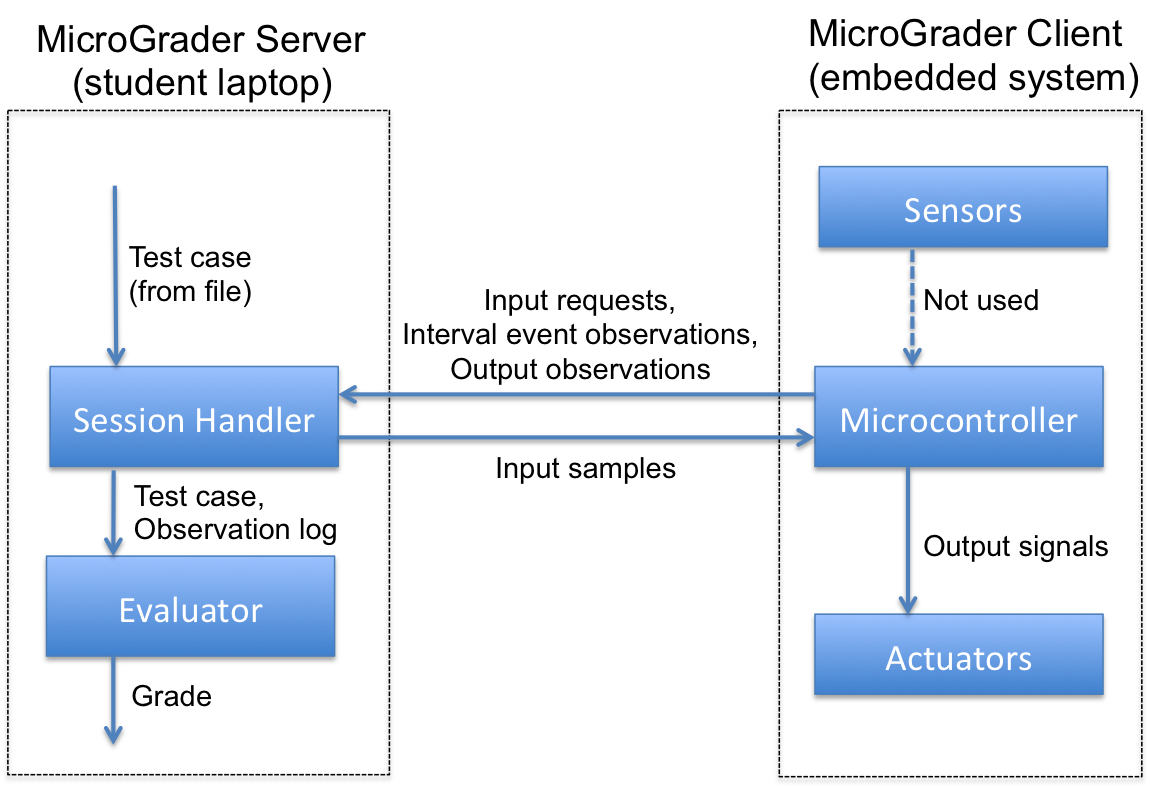
\includegraphics[scale=0.8]{test-mode.png}
\caption{Block diagram of MicroGrader in test mode.}
\label{fig:test-mode}
\end{figure}

TODO: describe timestamp definition (embedded system clock is master).  Also describe message contents in some reasonable detail

\subsection{Platform agnosticism}
TODO: describe why platform agnosticism is good

TODO: describe why Python 3 for server makes us agnostic

TODO: describe why reference client is Teensy-based

TODO: describe how thin client makes us more agnostic


\subsection{Two-stage testing}
Evaluation of a student's system occurs via a two-stage process.  First, the MicroGrader server and the embedded system engage in an interactive session to determine how the embedded system responds to test inputs.  The second stage assesses these responses and determines an overall score.

In the interactive stage, the server loads the relevant test case and waits for the client to connect.  Once the client connects, the server processes each message from the client and sends the appropriate response.  There are, broadly speaking, two types of message from the client to the server: observations and input requests.

If the message is an observation, such as an embedded system output or an important internal event, the observation and its timestamp are logged.  TODO: in addition, each input frame's conditions are updated live.  TODO: respond or not?

If the message is a request for an input value, TODO: paragraph

TODO: paragraph about test case end condition

In the evaluation stage, the MicroGrader server considers all the activity that occurred during the interactive session.  MicroGrader scans through the activity log in order to:

\begin{itemize}
\item Determine the time at which each evaluation point's condition was met, if it was met at all.  This allows for a point's relative time interval to be converted to an absolute time interval.
\item Reconstruct all the output signals.  Recall that we assume that each the output on each channel holds until the next output on the same channel.
\end{itemize}

Each evaluation point is examined and evaluated.  Refer back to section \ref{sec:eval-point} for details.  If an point's condition was never met, then that point automatically evaluates to \texttt{false}.  The boolean results of each evaluation point are aggregated into an overall score, as per TODO: section ref.


TODO: edit paragraph MicroGrader is \textbf{not} designed to gracefully handle errors.  If something goes wrong with the communication between the server and the client, or the client sends an invalid request, the session ends immediately and the test fails with an error message.  Similarly, if results of the session cannot be evaluated in the evaluation stage, the test automatically fails with an error message.  These situations are typically indicative of a malformed test case or a software bug that is not the student's responsibility.  Course staff should immediately address these types of issues.

\subsection{Reporting results}
For grading purposes, we only care about the numeric final score.  A student, however, would be well served by examining a rich and readable description of the test results.  In the event that a student does not receive full credit, this description should make it clear which points evaluated to \texttt{false} and why.

Specifically, for each evaluation point, the student can see:

\begin{itemize}
\item A text description of all the attributes of the point.
\item Whether that point evaluated to \texttt{true} or \texttt{false}.
\item A summary of the observed values on the point's channel in the point's interval.  This summary is comprised of:
\begin{itemize}
\item The unique values observed during the interval.
\item Whether or not each of those values was correct (as determined by the check function).
\item The portion of the interval for which each of those values was observed.
\end{itemize}
\end{itemize}

Some values do not lend themselves to a textual description.  For example, screen images (a very common type of output), are not easily converted to text.  To handle this, MicroGrader saves all screen images as image files in a special directory, and the text description of those images is just the file path.

For further readability, test results can be summarized somewhat more succinctly by only giving the full details for evaluation points that evaluate to \texttt{false}.  For points that evaluate to \texttt{true}, an abbreviated description can be used instead.  Students have access to both the full results and summarized results.

We considered a number of ways of reporting results to some online courseware (e.g. EdX, Coursera, etc.).  In the end, we chose a simple but effective solution, inspired by UT Austin's Embedded Systems course on EdX.  Students receive an individualized codeword for each test through the online courseware, and enter that codeword into MicroGrader.  When MicroGrader runs a test, the student's score is combined with that codeword and hashed.  The student can then copy that hash back into the courseware.  Since the number of possible scores is limited (scores are limited to four digits of precision), it's easy for the online courseware to determine the student's score.  This solution discourages cheating without requiring direct communication between MicroGrader and online courseware.  To further discourage cheating, courses could require students to upload their solutions to the online courseware for later reference.


\subsection{Screen analysis}
TODO: copy over and edit, add tons of pics (just use numpy to generate)

\subsection{Configurability and defaults}
MicroGrader is designed to be as configurable as possible.  This manifests itself in a variety of ways.  Test cases themselves are highly configurable, as described earlier.  Furthermore, certain design decisions were made in order to make MicroGrader compatible with as many embedded platforms as possible.  For example, it makes no assumptions about the resolution at which to discretize analog values.  Any request for an analog input or observation of an analog output comes packaged with information about the desired range and resolution of the analog quantity.

Later, it will be possible to add additional data types, beyond the built-in ones, without changing the source code.  The easiest way to do this is by importing serialized \footnote{https://docs.python.org/3/library/pickle.html} Python objects that include implementations of all the functions a data type needs to have.  The minimum functions for a new data type are: serialization, deserialization, and a definition of the equivalence operator.

The high level of configurability could potentially make it difficult for an instructor to use MicroGrader.  Therefore, wherever possible, reasonable defaults are included.  For example, consider the aggregator function, which maps a list of evaluation point results to a score.  By default, each channel uses a ``proportional" aggregator function, where the score is just the fraction of points that evaluate to \texttt{true}.  An instructor could replace this with any valid aggregator, such as an ``all-or-nothing" function which returns 1 if all points evaluate to \texttt{true} and 0 otherwise.







\newpage
\section{Technical design (deprecated)}
\subsection{Overall architecture}
\label{sec:architecture}
MicroGrader uses a client-server model.  The server is not a internet server, but rather a Python program running locally on a student's laptop or desktop machine.  That program connects to the client -- namely the embedded system being evaluated -- via USB serial.  The client is a thin wrapper of certain aspects of the embedded system's I/O functionality, which allows the server to ``drive" system inputs and observe results.

This key design choice stemmed from a desire to change the execution of an embedded program as little as possible.  A lightweight approach on the embedded side reduces the chances of incorrect evaluations (both false positives and false negatives).

\subsection{MicroGrader client}
The embedded client has two modes of operation.  In \textit{test} mode, we need to inject pre-defined inputs into the system instead of taking real input readings.  The software, in lieu of taking a real reading, makes a request via USB serial to the server, which responds with the proper pre-defined input value.  In the current reference implementation of the client, requests are blocking -- the embedded system will wait for a response if it expects one.  Currently, MicroGrader only supports one request ``in-flight" at a time.

For system outputs, the client really does produce the output (e.g. a digital write, or displaying something on a screen).  In addition to producing that output, the client reports the output to the server, for later evaluation.  The client also reports certain other system events, such as the beginning of program execution and various Wifi activity.

The other mode of operation on the client-side is \textit{inactive} mode.  In this mode, the client makes no request to the server whatsoever.  That is, the program should operate completely normally.  Inputs are read from the actual sensors, and outputs are not reported.  This mode allows students to experiment with an in-progress assignment without worrying about the grader.

The exact data that comprises client requests and reports varies depending on the type of request or report.  The communication protocol is detailed in Appendix A.  One commonality of all requests and reports is an integer timestamp, in milliseconds.  The server will trust this timestamp, and doesn't keep track of its own time during a live test.

Ideally, the functionality of the MicroGrader client should wrapped in a library and should mostly be invisible to the student writing code ``on top" of that library.  It may also be necessary to modify existing libraries that handle I/O functionality.  Details about the way this is accomplished in the reference implementation (for Teensy) can be found in Appendix B.

\subsection{MicroGrader server}
The MicroGrader server does the heavy lifting.  It is responsible for interpreting a test case, and using that test case's information to respond promptly and correctly to requests from the client.  We described the details of how a test case specifies input values in sections \ref{sec:static-inputs} and \ref{sec:frames}.  The server is also responsible for observing the system outputs and grading them according to the test case's specification.  The client has no knowledge of the whole test case, it only knows the server responses to its requests.

In the current implementation of the MicroGrader, all of the code is written in Python.  This language was chosen due to its ease of development and flexibility with data types.  Importantly, functions are first-order objects in Python which makes the implementation of a test case much easier (after all, a test case includes aggregator functions and check functions).  Python's popularity make it more convenient for others (especially time-strapped course professors and TAs) to understand and potentially extend the MicroGrader code base.

\subsubsection{Screen analysis}
As previously mentioned, binary (i.e. no partial intensities) monochrome screens are a built-in type.  MicroGrader also includes some utilities for working with such outputs, which are represented as a 2D array of binary values.  Specifically, these utilities help instructors build sensible check functions for this type of value.  After all, exact pixel-by-pixel screen matching is often not a reasonable requirement for students.

MicroGrader includes a built-in distance metric for binary monochrome screens.  It's basic functionality is simple: for two screens of the same dimensions, the distance between them is the number of pixels that do not match.  In practice, this fails to identify two screens that are very similar, but slightly shifted relative to one another.  Therefore, MicroGrader's distance metric allows the user to specify a maximum allowable shift of one screen relative to another, in any direction.  The distance is the \textbf{minimum} number of mismatched pixels.  Essentially, the function tries all allowable shifts and picks the best one.  Yet another built-in function checks that if a screen is significantly closer than a blank screen to a given reference screen.  After all, a blank screen might match a large number of pixels but isn't very close in terms of informational content.

Many assignments involving a screen are text-based.  That is, the screen is expected to contain printed text.  To that end, MicroGrader includes functionality to extract the text from the screen.  Various OCR engines were considered, but none worked acceptably well due to the tiny size of many fonts used in such contexts (potentially 5x7 pixels or smaller).  Instead, MicroGrader looks for rectangles on the screen that match the exact bitmap of a character.

There are a few downsides to this text extraction approach.  First, any noise in the image or overlying element makes extraction impossible.  Furthermore, fonts must fixed-width.  This isn't a fundamental constraint of this technique, but it does massively help performance since the algorithm only has to consider rectangles of a specific size.  The biggest issue is that MicroGrader needs to know the bitmap for each character in the font.  Since its sometimes not easy to find detailed information for embedded fonts, MicroGrader includes a utility to ``record" the character bitmaps of a font using the actual screen output.













\newpage
\section{Limitations}
Although MicroGrader is well-suited for grading many types of microcontroller projects, there are limitations that any instructor using this tool should know about.

\subsection{Latency}
In order to implement its side of the protocol, embedded clients must do some work.  Effort has been made to minimize this, but this issue nevertheless makes MicroGrader unusable for projects that have very sensitive timing, or that involve performing I/O operations at high frequencies.  In \textit{test} mode, the latency of reading an input is often orders of magnitude higher than in \textit{inactive} mode.  The embedded client must wait for the MicroGrader server to process and respond to a request for an input value.  Most of the latency is fundamentally due to the round-trip latency of the USB protocol, and due to the firmware on the server machine.

The latency issue makes is impossible for MicroGrader to examine raw communication channels such as UART, I2C, or SPI, or to inject values into those channels at a reasonable rate.

The specific constraints depend on the platform.  In building the reference implementation for Teensy, I observed that round-trip latency for relatively small messages ($<100$ bytes) was about a millisecond.  Therefore, the upper bound for the input sampling rate is around 1 KHz.  This is fast enough for many assignments that involve ``human" time scales, but woefully insufficient in other cases, such as audio sampling.

\subsection{Point-by-point evaluation}
Our \textit{evaluation point} model inherently forces a test case to independently evaluate points of an output signal.  For any given interval, there is a single expected value.   More sophisticated correctness metric, involving the entire output signal at once, aren't possible in this framework.  For example, we cannot use \textit{evaluation points} to determine the cross-correlation between the observed output signal and an expected output signal.

\subsection{Step-wise constant restriction}
MicroGrader assumes that the embedded system's outputs remain constant until the next output is observed.  While a step-wise constant function can approximate any step-wise continuous function to arbitrary precision, this can put an unacceptably high burden on the embedded client.  For example, both Arduino and Teensy have built-in functionality for creating square wave signals of a specified frequency for a specified duration, using a single user-facing instruction (\texttt{tone(pin, frequency)} or \texttt{tone(pin, frequency, duration)}).  In order for the embedded client to properly inform the server about the square wave signal, it would have to send a message on every rising and falling edge.  It is not possible, in a single message, to inform the server about the square wave that is being produced.

\subsection{Derived outputs}
\label{sec:derived-outputs}
In many systems, the embedded device produces outputs that serve as inputs to some physical plant, which then produces the outputs we actually care about.  For example, a microcontroller might drive the voltage across the terminals of a motor, connected to a wheel.  Perhaps we care only about the position of the wheel, not the motor's terminal voltage.  Even under the assumption that the motor's angular velocity is proportional to the terminal voltage, and the motor responds instantaneously, we would have to integrate the microcontroller's output to derive the pertinent physical output.

It is currently impossible to evaluate derived outputs like this using MicroGrader (unless the derived output is zeroth order linear function of the microcontroller's output).  In a later version, MicroGrader will include the ability to add a custom physical model to convert the raw output into a derived output.

\newpage
\section{Automatic Test Generation}
\label{sec:scaffold}

Using CAT-SOOP as a TA for MIT's 6.S08, the process of building test cases is a quick and convenient one.  An important convenience is the ability to only specify inputs for test cases.  CAT-SOOP uses a staff solution to generate the correct outputs for those specified inputs.  MicroGrader takes this philosophy one step further: it is possible to automatically generate a test case, including the desired system inputs, using a functioning staff solution.

\subsection{Re-examining Wikipedia Scroller}
Let's refer back to the Wikipedia Scroller exercise described in section \ref{sec:wiki-scroller}.  MicroGrader is capable of grading this assignment in a manner similar to a human grader.  It injects a representative sequence of inputs, and then checks to see that each expected output is observed on the screen at the correct time.

It would be fairly tedious, however, to manually construct a test case for this with MicroGrader.  An instructor would have to specify the entirety of the accelerometer input signal with exact timestamps, as well as the button input with exact timestamps.  Both of these inputs change values about a dozen times.

Constructing the evaluation points would be arduous as well.  The OLED changes at least 28 times in the above example.  While not all of these necessarily require checking, many of them do.  Even with MicroGrader's text extraction feature, it took quite a while for me to build a reasonable set of evaluation points.   Clearly, this process could use some further automation.

\subsection{Recording a reference solution}
In order to obtain a recording a correctly implemented solution, we use introduce a third client-side mode, which we'll call \textit{recording} mode (the first two modes were \textit{test} and \textit{inactive} modes). 

Recording mode is quite similar to test mode, with one key difference.  In test mode, input sampling is replaced with requests to the MicroGrader server.  In recording mode, by contrast, input sampling occurs normally (i.e. sensors are actually used).  Those real-world values are then reported to the MicroGrader server.

An instructor with a working solution can switch the client to recording mode, perform some set of tasks that fully demonstrate the functionality of the system.  Meanwhile, the MicroGrader server makes a full record of this activity, including both inputs observed and outputs generated.  That activity log is then used to programmatically construct a test case.

\subsection{Constructing a test case}
Completely generating a test case from a log along turns out to produce poor results.  There are plenty of ambiguities in terms of how the instructor might want to the assignment to be graded.  MicroGrader uses a lightweight data structure called the \textit{scaffold} to allow for instructors to specify these preferences.  The scaffold and activity log, when combined, can be used to produce a full test case.

\subsubsection{Data structure: Scaffold}
The two primary aspects of the \textit{scaffold} are \textit{frame templates} and \textit{point templates}.

Frame templates arise out of the need to specify which intervals of time are relevant from a grading standpoint.  Specifically, the generated test case needs to know when to ``care" about the system outputs, and when to ignore them (e.g. while waiting for a internet request to resolve, or while waiting to get a GPS fix).  The relevant intervals might comprise only a small portion of the total operation of the system.

The most important two components of a frame template are the \textit{start condition} and \textit{end condition}.  These are instances of our familiar \textit{condition} data structure, and will serve as the start and end conditions for the frame that will be generated.  Refer back to section \ref{sec:frames} for more information.

In our Wikipedia Scroller exercise, we can use a scaffold with two frame templates for the evaluation procedure previously outlined.  The first frame could start when system initialization is complete, and end when the first Wifi request occurs.  The second frame could start when the first Wifi response arrives, and end when the recording ends (I usually end recordings by just unplugging the client system).  This two-frame structure allows the test case to ignore the variable latency period of time when the Wifi request is awaiting a response.  After all, the length of this time period shouldn't be relevant in determining the correctness of a student's solution.  If we tried to use one frame for this whole evaluation, the student solution's timing after the variable-latency event would certainly mismatch the staff solution's timing.

The other major aspect of a scaffold is the set of \textit{point templates}.  For each output channel, a point template is defined.  This template will indicate how the instructor wants each \textit{evaluation point} to be configured.

The three components of a point template are:

\begin{itemize}
\item Check Function
\item Required Portion
\item Time Interval
\end{itemize}

Using these point templates, we can specify aspects we want all evaluation points (for a certain channel) to share.  For example, an instructor might want a special check function for values on the \textit{Screen} channel.  Perhaps in the case of our Wikipedia Scroller, that check function would verify that the text of the expected value and observed value are the same (regardless of where on the screen that text occurs).  Furthermore, an instructor might want to impose a strict evaluation of a specification, requiring that student's solutions match the staff solution for a high portion of the time interval.  On the other hand, an instructor may opt for a looser evaluation and reduce the required portion.

The time interval component of the point template is somewhat difficult to describe without a worked example.  We'll get into that in section \ref{sec:using-point-templates}.

\subsubsection{Constructing test inputs}
We construct a full set of input signals for each frame. First, the entire activity log is scanned to determined the times at which the start and end condition for each frame template were fulfilled.  We only generate a frame from a frame template if both the start and end condition were met, and the start condition was met first.

For each generated frame, we consider all input values recorded by the client between the times that the start and end condition were met.  We convert the absolute times of these recorded inputs to relative times by subtracting the time at which the start condition was met.

One issue we haven't addressed yet is interpolating the recorded inputs.  After all, those represent a sample of a continuous signal.  MicroGrader gives instructors several options as to how to interpolate the sampled input -- the following methods are all supported.  For the sake of clarity, consider a value recorded at time $t_n$.  The previous recording occurred at time $t_{n-1}$ and the subsequent recording occurred at time $t_{n+1}$.

\begin{itemize}
\item Start: a recorded value holds in the interval $[t_n, t_{n+1})$
\item End: a recorded value holds in the interval $(t_{n-1}, t_n]$
\item Mid: a recorded value holds in the interval $[(t_{n-1} + t_n)/2, (t_n + t_{n+1})/2)$
\item Linear: perform linear interpolation with a specified resolution between each sample.  Note that this doesn't work for certain input types (namely digital inputs).
\end{itemize}

\subsubsection{Constructing evaluation points}
\label{sec:using-point-templates}
Just as with input generation, we first determine which frame templates generate a frame by determining the times at which their conditions were fulfilled.  Again, for each frame, we consider the outputs on all channels that were reported between the fulfillment of the frame's start and end conditions.

For each (frame, channel) pair, we create a set of evaluation points.  Specifically, we create a new evaluation point each time the output value changes on that channel.  It is important to note that repeated output reports of the same value have no effect.  For example, if the voltage on a pin is currently 0, and the microcontroller executes a command that sets the voltage on that pin to 0 again, that is functionally equivalent to doing nothing.  The change in the value is all that matters.

In constructing each evaluation point, we can easily determine the channel.  The expected value is equal to the observed value, since this is a staff recording and we consider its outputs to be canonically correct.   For the point's check function and required portion, we use the values for the point template for this channel.  For the point's condition, we use the start condition of the frame we are currently considering.

To complete our construction of an evaluation point, we need to specify the time interval.  The time interval is generated using a combination of the time interval of this channel's point template, and the activity log.  Specifically, the template time interval is not relative to the fulfillment of the frame's start condition, but rather relative to the time at which the output was reported.  So if the template time interval is \texttt{(0, 100)}, the frame's start condition was met at $t=1000$, and a new output is reported at $t=1500$, then the evaluation point for this output will have an interval of \texttt{(500, 600)}.  Recall that an evaluation point's time interval is relative to the point's condition being met.  More generally, if the template interval is $(t_{start}, t_{end})$, the condition is met at $t_{cond}$ and the output is reported at $t_{output}$, the evaluation point's interval will be $(t_{output} - t_{cond} + t_{start}, t_{output} - t_{cond} + t_{end})$.

A fixed-width time interval, like the one mentioned in the previous paragraph, is not very useful in a template.  Typically, the length of the interval should be relative to the length of time for which the output was sustained in the correct solution.  A fixed interval of width 100 milliseconds would be unreasonable if the correct solution sustained that output for only 50 milliseconds.  Furthermore, it would be too lenient if the correct solution sustained that output for 5000 milliseconds.

To give instructors the ability to tune the width of evaluation intervals in a dynamic way, elements of the template time interval can be mathematical formulae (represented in string form) rather than just integers.  In particular, this string can include a special variable, \texttt{T}, representing the length of time for which the recorded output was sustained.  For example, a point template might have the time interval \texttt{("0.2*T", "0.8*T")}, which indicates that the evaluation point's interval should cover the middle 60\% of the observed interval. 

\subsection{Auto-generated test case for Wikipedia Scroller}
For an instructor to automatically generate a test case, he or she would first have to record a correctly implemented system performing the relevant operations (in our example, creating the query string ``cat" and fetching the relevant information from the internet).  For this assignment, a fairly simple scaffold would do.  Consider the following possible scaffold:

The scaffold has has templates specifying the beginning and end of two separate frames.  The first frame should begin upon system initialization and end upon the first internet request.  The second frame should begin upon the response to that internet request, and end a few seconds afterward.  For point templates, the default point template suffices, with a time of interval of \texttt{("0.2*T", "0.8*T")} as mentioned above.  This gives a bit of leniency on the exact timing of state transitions in the student's solution.

With this simple scaffold, and the recording of the staff solution, MicroGrader can generate a test case that checks for all the outputs that a human grader would look for.  Furthermore, the test case's use of two separate frames ensures that students would not be penalized for internet requests that are quicker or slower than the one in the original recording.

\subsection{Resolving ambiguous cases}
\label{sec:resolve-ambiguity}
There is a major potential problem when recording a canonically correct staff solution.  First, the reconstruction of the input signals from the recorded input samples is inevitably imperfect.  Staff members should keep this in mind designing their solutions.  Specifically, it's a good idea for the staff solution to sample (and therefore report) the input at a relatively high frequency even if such a high frequency isn't necessary for a correct implementation.  This will give the MicroGrader server a maximally high resolution view of the inputs that the staff member physically created.

Even if we could, somehow, record an infinitely high resolution input signal, some recordings could have problems.  Namely, the desired system output could be ambiguous for that particular input signal.  This commonly happens in edge cases.  It is possible to make the specification stricter to avoid such ambiguities, but that might be undesirable from a pedagogical standpoint.  The instructor's solution would record one acceptable output.  As a result, other acceptable outputs would be seen as incorrect.

A subsequent version of MicroGrader will include tools for instructors to avoid ambiguous inputs.  Specifically, these tools will allow instructors to edit recordings of input signals.  Presumably, an instructor would be able to remove any ambiguities.  After editing, these new input signals would be injected back into the instructor's embedded system to record the unambiguously correct output.


\newpage
\section{Future Work}
This thesis is being submitted with the described functionality, but many of the aforementioned shortcoming can be overcome.  A version 2.0 of MicroGrader is under construction, and it will include the following improvements.

\subsection{Custom data types}
In the current implementation of MicroGrader, adding custom data types requires modifying the source code.  In the next version, it will be possible to specify a custom data type in a separate file.  The file will include the name of the data type, as well as the implementations (in Python) of certain necessary functions.  Namely, there must be functions to serialize and deserialize the data type, and the equality operator must be implemented.

\subsection{Timing flexibility}
It is currently difficult for instructors to have loose timing specifications, since \textit{evaluation points} inherently have a pre-determined time interval.  The only flexibility is picking a condition to which that interval is relative.  In the next version of MicroGrader, the data structure for test cases will be augmented such that an instructor can give different sorts of timing specification.  For example, an instructor can specify that a certain sequence of outputs must occur in a certain order, regardless of timing.  It will also be possible to put requirements on the length of time for which an output occurs, regardless of exactly when it occurs.

\subsection{Editing recordings}
As mentioned in section \ref{sec:resolve-ambiguity}, a set of tools will be included in the next version of MicroGrader to facilitate some manual editing of recordings of a instructor's correctly implemented system.  This will help create test cases that are unambiguous.  Ideally, these tools will also help an instructor programmatically edit a recording.

\subsection{Dynamic values}
Certain ``correct" values are not determined at the time the test case is created.  For example, the Wikipedia Scroller assignment has an output that involves the current text on Wikipedia.org.  The next version of MicroGrader, will include a ``place-holder" data type.  This placeholder will be a function that runs at evaluation time to generate the correct value.  In the Wikipedia Scroller case, the placeholder would fetch the correct text from Wikipedia.

\subsection{Second order outputs}
As mentioned in section \ref{sec:derived-outputs}, it is sometimes desirable to measure an output that is not directly generated by the microcontroller, but rather is some transformation of an output generated by the microcontroller.  In the next version of MicroGrader, instructors will have the ability to add a custom physical model to convert the microcontroller's outputs to a derived output (e.g. converting a motor voltage to the position of an attached wheel).

\newpage

\section{Appendix A: Client-server protocol}
\label{sec:protocol}
All client-server communication occurs over a USB connection.  All multi-byte integers are transmitted in a little-endian fashion.  In general, we refer to a message from the client to the server as a \textit{request}.  Some requests result in server-to-client \textit{response}.

All messages consist of a header and a body.  The header contains important information about the request or response, and specifies the length of the body. Thus, our protocol requires no termination byte.  A message is considered complete once the expected number of bytes is received.  As a result, all message bodies must have the specified length, or further communication will fail.

The basic structure of a request is as follows:

\textbf{request ::= $<$request header$>$$<$request body$>$}

\textbf{request header ::= $<$uint8 code$>$$<$uint32 timestamp$>$$<$uint16 body length$>$}

\noindent The most significant bit of the request code determines whether or not the server should send a response.  If the bit is 0, a response should be sent.  If the bit is 1, a response should be omitted.  The lower seven bits of the code determine the type of request, and therefore, how the request body should be interpreted.  The structure of the request body depends on the particular type of request.  The timestamp is measured in milliseconds, and the body length is measured in bytes.

The basic structure of a response is as follows:

\textbf{response ::= $<$response header$>$$<$response body$>$}

\textbf{response header ::= $<$uint8 code$>$$<$uint16 body length$>$}

\noindent The second-least significant bit of the response code indicates whether or not an error occurred with the most recent request (1 indicates an error occurred, 0 indicates success).  The response body for an error response is always empty.

The least significant bit indicates if the current session is complete (1 indicates yes, 0 indicates no).  The server disconnects immediately after sending a response indicating the session is complete.  Once again, the body length is measured in bytes.  Notice that the server does not include a timestamp in the response header.  The structure of the response body depends on the type of request to which the response corresponds.

Broadly speaking, there are three kinds of requests: inputs, outputs, and events.

\subsection{Inputs}
Input requests are typically used to ``inject" pre-determined test values, in place of true sensor readings.  Alternatively, input requests can be used to record observed sensor values on an instructor's system, for the purpose of building tests.  The following table describes the request bodies for input requests.

\begin{center}
\begin{tabular}{l l l}
code & name & request body \\ \hline
0x20 & Digital Read & $<$uint8 pin$>$[$<$uint8 value$>$] \\
0x22 & Analog Read & $<$uint8 pin$>$$<$analog params$>$[$<$int32 value$>$] \\
0x30 & Accelerometer & $<$analog params$>$[$<$int32 x value$>$$<$int32 y value$>$$<$int32 z value$>$] \\
0x31 & Gyroscope & $<$analog params$>$[$<$int32 x value$>$$<$int32 y value$>$$<$int32 z value$>$] \\
0x32 & Magnetometer & $<$analog params$>$[$<$int32 x value$>$$<$int32 y value$>$$<$int32 z value$>$] \\ \hline
\end{tabular}
\end{center}

\vspace{5mm}

If the optional value or values are included, this message is passing recorded sensor readings from the client to the server.  In that case, the body of the response (if there is a response) is empty.  

If the optional values are not included, this message is requesting test values.  In that case, the body of the response (if there is a response), is just the requested values.  For digital reads, the response is a single byte containing a 0 or a 1.  For analog reads, the response is a 32-bit integer.  For the accelerometer, gyroscope, and magnetometer requests, the response is a sequence of three 32-bit bit integers representing the x-value, y-value, and z-value respectively.

\subsubsection{Value Encoding}
Encoding for digital values is simple: a single byte containing the value 0 or 1.  For analog values, however, MicroGrader uses a system by which the client decides how an analog value becomes discretized.  In particular, the client specifies the \textit{analog params} which are defined as follows:

\footnotesize
\textbf{analog params ::= $<$int32 min bin$>$$<$int32 max bin$>$$<$int32 min value$>$$<$int32 max value$>$}
\normalsize

\noindent These parameters indicate that the physical quantity in the range (min value, max value) should be mapped to the range (min bin, max bin) for discretization.

To illustrate, let's examine the behavior of the Teensy client for analog read requests.  It uses the values 0 and 3300 for min value and max value respectively.  These represent the minimum and maximum voltages, in millivolts, that the Teensy's analog-to-digital converter (ADC) can process.  For min bin and max bin, the values depend on the Teensy's current analog resolution.  If the resolution is 10 bits for example, the Teensy client would use the values 0 and 1023 for min bin and max bin.

Let's suppose the Teensy makes a request for an analog read using these parameters, and the server observes that the true value to ``inject" is $x$.  Let $b_{\text{min}}$, $b_{\text{max}}$, $v_{\text{min}}$, and $v_{\text{max}}$ represent the min bin, max bin, min value, and max value respectively.  The server must convert the value $x$ to a ``bin number", $y$, in accordance with the given parameters:

$$y = \left \lfloor b_{\text{min}} + \frac{x_{\text{bound}}-v_{\text{min}}}{v_{\text{max}}-v_{\text{min}}} * (b_{\text{max}}-b_{\text{min}}) \right \rfloor$$

where

$$x_{\text{bound}} = \min(v_{\text{max}}, \max(v_{\text{min}}, x))$$

The server responds with the value $y$.  This example discussed a true input request for injecting a value.  For input ``recordings", the value supplied by the client should also be the bin number as described by the above formula (typically this math would be calculated in hardware by the ADC).

\subsubsection{Units}
The units for analog requests are not specified.  There is no built-in unit for the relevant physical quantities (namely voltage, acceleration, angular velocity, and magnetic flux density).  The client implementation and the constructed test cases just need to be consistent.  For example, the reference Teensy client implementation uses millivolts for voltage, and any test cases written for this client should use values expressed in millivolts.

\subsection{Outputs}
Output requests aren't really ``requests" in the traditional sense.  They are used to report outputs to the server.  The following table describes the request bodies for output requests.

\begin{center}
\begin{tabular}{l l l}
code & name & request body \\ \hline
0x21 & Digital Write & $<$uint8 pin$>$$<$uint8 value$>$ \\
0x23 & Analog Write & $<$uint8 pin$>$$<$analog params$>$$<$int32 value$>$ \\
0x41 & Screen & $<$tile$>$* \\
%0x42 & Screen Tile & $<$uint8 x position$>$$<$uint8 y position$>$$<$tile$>$ \\ \hline
\end{tabular}
\end{center}

\vspace{5mm}

If the client expects a response, the body of the response is empty.  The encoding of values for digital writes is the same as for digital reads (a single byte, 0 or 1).  The encoding of values for analog writes is the same as for analog reads.  Recall that the value reported is a ``bin number".

\subsubsection{Screen Encoding}
Since the built-in screen type is a monochrome display, in which each pixel is on-or-off, our screen is essentially a bitmap.  We represent each pixel using a single bit.  Our encoding for the screen is inspired by the U8x8 embedded library \footnote{https://github.com/olikraus/u8g2/wiki/u8x8setupcpp}, and it makes it simple for embedded clients to transmit screen information if their display libraries are U8x8 compatible.

We code encode the screen as a collection of 8x8 \textit{tiles}.  The entire bitmap for a tile is contained in an unsigned 64-bit integer.  The most significant byte of the 64-bit integer encodes the leftmost column of the tile.  The next-most significant byte encodes the second-to-leftmost column of the tile, and so forth.  Within a 8-pixel column, the most significant bit represents the state (on or off) of the top pixel, the second-most significant bit represents the state of the pixel below that, and so forth.  In our terminology, the leftmost column has the coordinate $x=0$ and the topmost row has the coordinate $y=0$.  Therefore, the point $(0, 0)$ is the top-left corner of a bitmap.  When a tile is transmitted over serial, note that this unsigned 64-bit integer, like all our other multi-byte integers, are transmitted in a little-endian fashion.  So the lowest-order byte, representing the rightmost column of the tile, is transmitted first.

The screen can be considered a grid of non-overlapping tiles (though padding might be necessary so that tiles perfectly cover the entire screen.  When transmitting the screen, the tiles are transmitted by row, from top to bottom (lowest y-coordinate to highest y-coordinate.  Within each row, tiles are transmitted from right to left (highest x-coordinate to lowest x-coordinate).  Note that the Screen request does not specify the shape of the screen (just the overall number of tile).  Therefore, it is imperative that, before sending any Screen requests, the client informs the server of the screen shape using a ``Screen Init" request (see the section below).

\subsection{Events}
Event requests are similar to output requests in that they are used to report information to the server, not receive information from the server.  Responses to event requests have empty bodies, just as with output requests.  The following table describes the request bodies for event requests.

\begin{center}
\begin{tabular}{l l l}
code & name & request body \\ \hline
0x00 & Init & (\textit{empty}) \\
0x01 & Print & $<$uint8 char$>$* \\
0x40 & Screen Init & $<$uint8 width$>$$<$uint8 height$>$ \\
0x50 & GPS Fix & (\textit{empty}) \\
0x60 & Wifi Request & (\textit{empty}) \\
0x61 & Wifi Response & (\textit{empty}) \\ \hline
\end{tabular}
\end{center}

\vspace{5mm}

The Init request is sent when the embedded client initializes.  In addition, the Screen Init request is used upon initialization to inform the server of the width and height of the screen, as measured in 8x8 tiles.  The Print request is used to send custom text (ASCII-encoded) from the client to the server.  This is particularly helpful for debugging, since it is impossible to perform regular debugging via USB serial when MicroGrader is in use.

It is important to inform the server of certain events, especially ones that have highly variable latencies.  The GPS Fix request is used to inform the server that the client has acquired a GPS fix.  The Wifi Request request is used to inform the server that a internet request has been sent.  The Wifi Response request is used to inform the server that a internet response has been received.

\newpage
\section{Appendix B: Client implementation for Teensy}
\label{sec:teensy}
MicroGrader is built to be cross-platform and is should work with a wide variety of microcontrollers.  As of now, the client side of the communication protocol is implemented for only one microcontroller: the Teensy, an Arduino variant.  The key for any client implementation is to be as invisible to students as possible.  In the case of the Teensy implementation, students write implement projects in a \texttt{.ino} file, which has access to a built-in functions.  In order to properly implement the protocol, I wrote a library that overrides many of these built-in functions to perform the proper communication with the server.  The required changes to the student's \texttt{.ino} file are minimal.

At its core, the client consists of a communication library that interacts with the server.  It provides functionality for other libraries to send messages to the server; the core communication library adds the request header to the message.  If the request requires a response, the communication library waits, and processes, that response, and returns its contents.  If the request does not require a response, the communication library returns immediately after sending a request.

The Teensy includes built-in functions to send and receive data over USB.  The MicroGrader client for Teensy replaces the built-in \texttt{Serial} object with a wrapper object.  When in \textit{test} mode or \textit{recording} mode, any print statements made using \texttt{Serial} have no effect.  For cases where a student or instructor wishes to print some text for debugging, the library includes a \texttt{debug} function, which sends a Print message in accordance with the MicroGrader protocol.  When the client is in \textit{inactive} mode, \texttt{Serial} print statements work normally.  Therefore, students can use \texttt{Serial} print statements when not connected to the MicroGrader server, but they don't have to worry about those statements interfering with MicroGrader communication when actual testing is happening.

The fundamental general purpose I/O functionality (GPIO) is also wrapped.  This allows for recording GPIO events and for injecting test inputs from the host.  As with \texttt{Serial}\texttt{Serial}, the regular GPIO functions work normally when the client is in \textit{inactive} mode. 

For input from the inertial measurement unit (IMU), I modified the MPU9250 \footnote{https://github.com/sparkfun/SparkFun\_MPU-9250-DMP\_Arduino\_Library} library for Arduino/Teensy.  For output to a display, I modified the U8g2 \footnote{https://github.com/olikraus/u8g2/wiki} library for Arduino/Teensy.  If a course uses the Teensy, but uses different libraries for IMU input and screen output, the course staff must modify the source code of those libraries.  Specifically, those libraries need to request inputs from the MicroGrader server when appropriate, instead of performing real sensor readings, and need to report information to the MicroGrader server when appropriate.  In practice, the code for doing this, with the help of the core communication library, is not complicated.

From a student's perspective, very few changes need to be made in order to run the MicroGrader client.  He or she needs to install the core library and the modified versions of the third-party libraries.  The line \verb+#include "MicroGrader.h"+ must be added to the top of the \texttt{.ino} file and an initialization function, \texttt{MicroGrader.begin()} must be called at the beginning of the Teensy \texttt{setup()} routine.

\newpage
\section{References}
TODO

\end{document}